\title{\vspace{160px} \textbf{\huge{Multimedia}} \\\vspace{17.5px} \LARGE{Homework 1}  \vspace{10px}}
\author{\href{https://github.com/imAlessas}{Alessandro Trigolo}}
\date{7 Maggio 2024}

\begin{document}

\maketitle\newpage

\tableofcontents
\listoffigures
\vspace{20px}
\newpage

\listoftodos\newpage


\section*{Introduzione}
Il linguaggio scelto per completare le richieste dell'homework è \texttt{Python}; all'interno del documento saranno presenti solo i punti salienti dello script, che comunque può essere ispezionato al seguente \href{https://github.com/imAlessas/computer-networks/blob/main/multimedia/hw-1/script/lossless_coding.py}{\texttt{link}}.
\todo{Inserisci introduzione dove spieghi l'obiettivo discuti brevemente come hai fatto il codice e dove trovarlo. Inserisci link a github etc}


\section{Codifica semplice} 
\todo{inserisci mini introduzione}

\vspace{15px}\subsection{Caricamento dell'immagine}
La prima richiesta dell'homework consiste nel caricare un'immagine a livelli di grigio oppure un'immagine a colori ed estrarne la luminanza, approssimabile come la media tra i tre canali di colori dell'immagine (\textsl{Red}, \textsl{Green} e \textsl{Blue}). Il frammento di codice seguente incontra esattamente le richeste della prima task dove, attraverso la funzione \texttt{imread} del modulo \texttt{matplotlib.image}, l'immagine viene letta correttamente ed, eventualmente, ne viene estratta la luminanza.

\begin{lstlisting}
    # Prepare to load the image
    img_file_name = "spiderman"
    img_extension = ".jpg"
    current_dir = os.getcwd()

    # path to reach the img
    path_to_img = os.path.join(current_dir, "multimedia", "hw-1", "script", "imgs") + "/"

    # loads the colored image
    gray_img = mpimg.imread(path_to_img +  img_file_name + img_extension).astype(np.int16)

    # extracts the luminance if RGB
    if gray_img[0][0].size > 1:
        gray_img = np.dot(gray_img[..., :3], [1, 1, 1]) / 3
\end{lstlisting}

\noindent Scegliendo un'immagine a colori è quindi possibile verificare il corretto funzionamento del codice, come mostrato nella figura \ref{fig:colored-grayscale} dove si è scelto come riferimento quella di \textsl{Spiderm-Man}.

\begin{figure}[h]
    \centering
    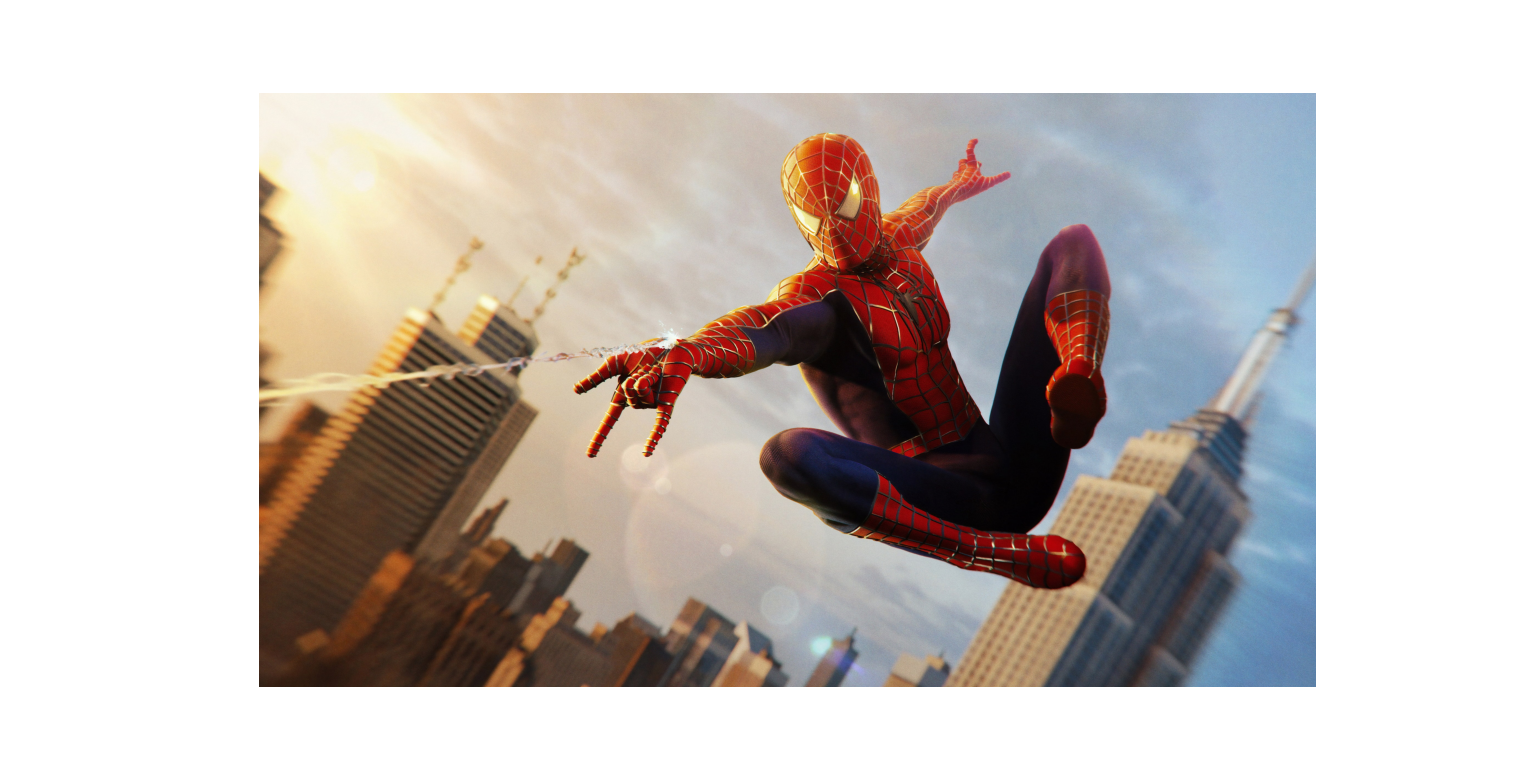
\includegraphics[width = .7\textwidth]{hw-1/report/imgs/colored.png}
    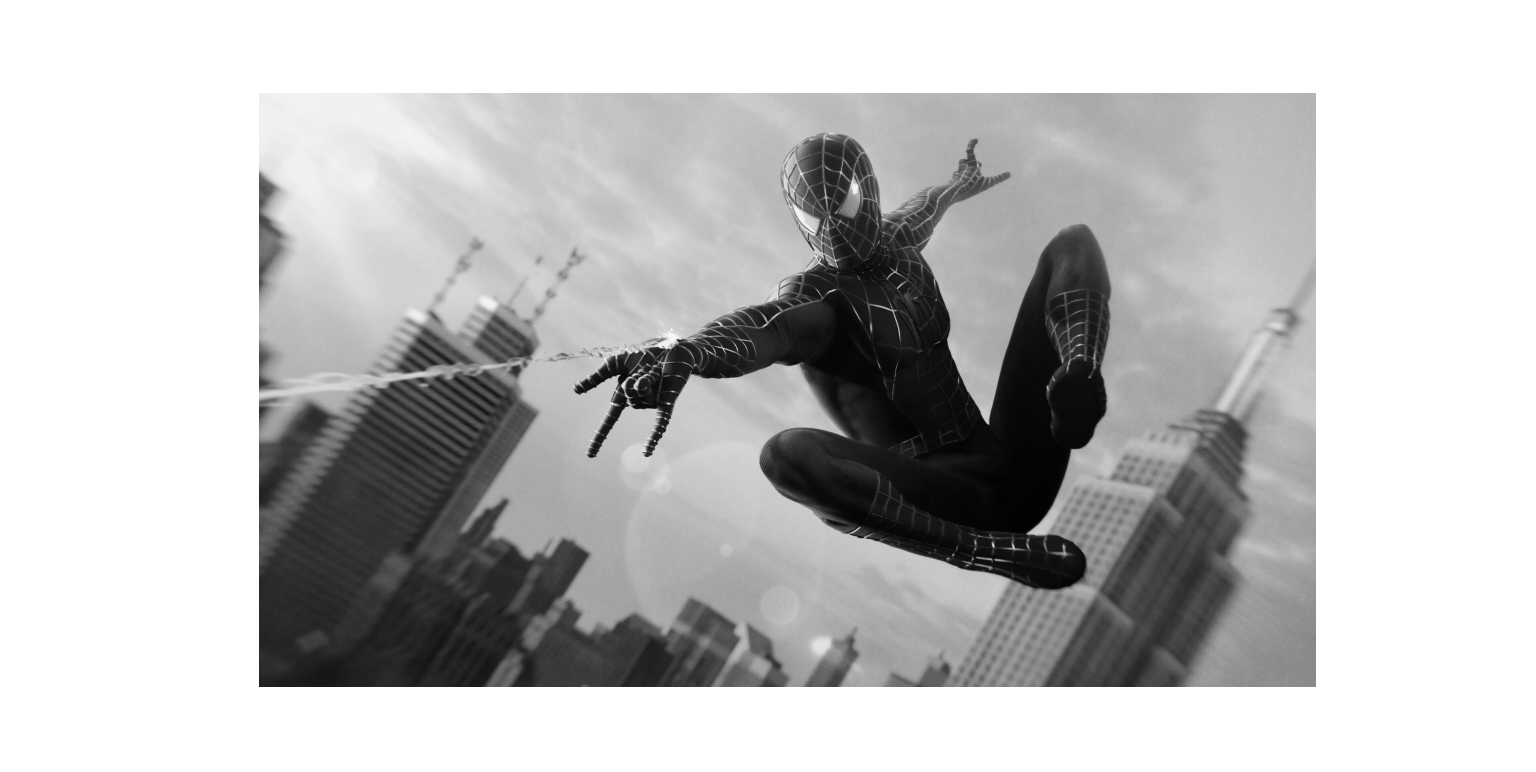
\includegraphics[width = .7\textwidth]{hw-1/report/imgs/grayscale.png}
    \caption{Estrazione della luminaza da una immagine a colori.}
    \label{fig:colored-grayscale}
\end{figure}



\subsection{Entropia dell'immagine}\label{img-entropy}
La seconda task dell'homework richiede di calcolare l'entropia dell'immagine in scala di grigi. L'entropia di una variabile aleatoria $X$ (in questo caso l'immagine) è definita come l'\textbf{informazione media} degli eventi della sorgente; l'informazione di un evento è descritta dalla funzione seguente:

\begin{gather*}
    I(X) = \log_2\left( \frac{1}{p_i} \right)
\end{gather*}

\noindent L'informazione media diminuisce all'aumentare della probabilità dell'evento $p_i$. Questo è ragionevole in quanto più un evento è imporbabile (quindi $p_i \to 0$) e più la sua informazione è alta ($I(X) \to +\infty$). Assumendo che gli eventi della sorgente siano indipendenti, l'informazione media si traduce nella seguente formula:

\begin{gather*}
    H(X) = E[I(X)] \, = \, \sum_{i = 1}^M p_i\log_2\left( \frac{1}{p_i} \right) \, = \, - \sum_{i = 1}^M p_i\log_2{p_i}
\end{gather*}

\noindent Dove con $M$ si indica il numero di elementi nell'insieme $X$. Questa formula si riassume nel seguente script, dove la variabile contenente l'immagine in bianco e nero viene trasposta e convertita in un vettore monodimensionale. In secondo luogo attraverso la funzione \texttt{numpy.histogram} vengono contate il numero di occorrenze per ogni valore di pixel. Successivamente, per calcolare la probabilità, si divide il numero di occorrezze per il numero totale di occorrenze, escludendo eventuali valori diversi da zero. Una volta calcolare la probabilità, attraverso le funzioni  \texttt{numpy.sum} e \texttt{numpy.log2} si ottiene il valore dell'entropia $H(X)$.


\begin{lstlisting}
    # flatten the transposed matrix to read pixels row by row
    raster_scan = np.transpose(gray_img).flatten()

    # count the occurrences of each pixel value
    occurrencies = np.histogram(raster_scan, bins=range(256))[0]

    # calculate the relative frequencies
    rel_freq = occurrencies / np.sum(occurrencies)

    # remove zero-values of probability
    p = rel_freq[rel_freq > 0]

    # compute the entropy
    entropy_x = - np.sum(p * np.log2(p))
\end{lstlisting}

\noindent Dopo aver eseguito lo script, l'entropia dell'immagine scelta è di \textbf{7.581 bpp}.



\vspace{15px}\subsection{Codifica con dizionario} \label{dictionary-coding}
La terza task chiede di utilizzare una compressione a dizionario, come \texttt{zip} nel caso di \textsl{Windows} per poi calcolare il \textsl{bitrate} risultante. Lo script necessario per soddisfare la richiesta è presentato nel frammento di codice sottostante. In particolare le prime righe si occupano di \textsl{"zippare"} il file mentre le istruzioni seguenti estraggono la dimensione dell'immagine compressa (in bytes). Infine nelle ultime linee del frammento di codice viene computato l'effettivo \textsl{bitrate} dividendo la dimensione del file compresso con la dimensione dell'immagine originale.

\begin{lstlisting}
    # change the current working directory to the directory containing the image
    os.chdir(path_to_img)

    # zip the image
    cmd = f"zip {img_file_name}.zip {img_file_name}{img_extension}"
    os.system(cmd)
    
    # get the zip bytes
    zip_bytes = os.stat(f"{img_file_name}.zip").st_size

    # get img size
    height, width = gray_img.shape
    img_size = width * height

    # get the birate
    zip_bitrate = zip_bytes * 8 / img_size 
\end{lstlisting}

\noindent Dunque, dopo aver eseguito lo script si ottiene il valore del bitrate, corrispondente a \textbf{1.329 bpp}. 



\vspace{15px}\subsection{Discussione risultati parziali}
Osservando il valore di entropia ottenuto nel punto \ref{img-entropy} si osserva che quest'ultima è molto vicina ad 8, indicando il fatto che l'immagine trovata, in ogni pixel, contiene 7.581 bit di  informazione su un limite massimo di di 8 bpp. Il motivo per cui tale valore non è esattemente 8 può dipendere dal fatto che l'immagine (figura \ref{fig:colored-grayscale}) contiene zone molto unifoirmi rispetto ad altre, per esempio il cielo e i grattacieli, i quali sono tutti della stessa tonalità di girgio e sono più o meno uniformi rispetto al personaggio raffigurato.

Il fatto che la compressione attraverso la codifica con dizionario abbia un bitrate di 1.329 bpp (punto \ref{dictionary-coding}) sta a signifcare che, nonostante l'entropia dell'immagine fosse alta, la compressione è riuscita a sfruttara in maniera ottimale la ridondanza dei dati, precedentemente puntaulizzata. Infatti si osserva che dividendo l'entropia iniziale con il bitrate ottenuto dalla codifica con dizionario si ottene un \textbf{tasso di compressione} di 5.706, che indica una compressione particolarmente efficacie, nonostante l'elevata entropia iniziale.



\vspace{15px}\subsection{Codifica semplice}\label{simple-coding}
La quinta richiesta dell'homework è quella di effettuare una codifica predittiva \textsl{semplice}. In particolare, data l'immagine, definita come un vettore chiamato $x(n)$, la codifica predittiva è definita come segue:

\begin{gather*}
    x(n) = 
    \begin{cases}
        128 \hspace{37px} \text{se } \, n = 0 \\
        x(n - 1) \hspace{15px} \text{altrimenti}\\
    \end{cases}
\end{gather*}

\noindent Di conseguenza l'errore di predizione $y(n)$ sull'immagine $x(n)$ è dato da:

\begin{gather*}
    y(n) = 
    \begin{cases}
        x(n) - 128 \hspace{37px} \text{se } \, n = 0 \\
        x(n) - x(n - 1) \hspace{15px} \text{altrimenti}\\
    \end{cases}
\end{gather*}

\noindent Tale codifica si traduce nel seguente codice Python, dove viene utilizzato il vettore \texttt{raster\_scan}, calcolato nel punto \ref{img-entropy}, contenete il vettore dell'immagine in scala di grigi.

\begin{lstlisting}
    # calculate prediction error
    simple_coding_error = np.concatenate(([raster_scan[0] - 128], np.diff(raster_scan.astype(float))))

    # plot error graph
    simple_coding_error_img = np.transpose(np.reshape(np.abs(simple_coding_error), (width, height)))

\end{lstlisting}

\noindent Dopo aver eseguito lo script soprastante si ottiene l'immagine mostrata nella figura \ref{fig:simple-coding}.
\begin{figure}[h]
    \centering
    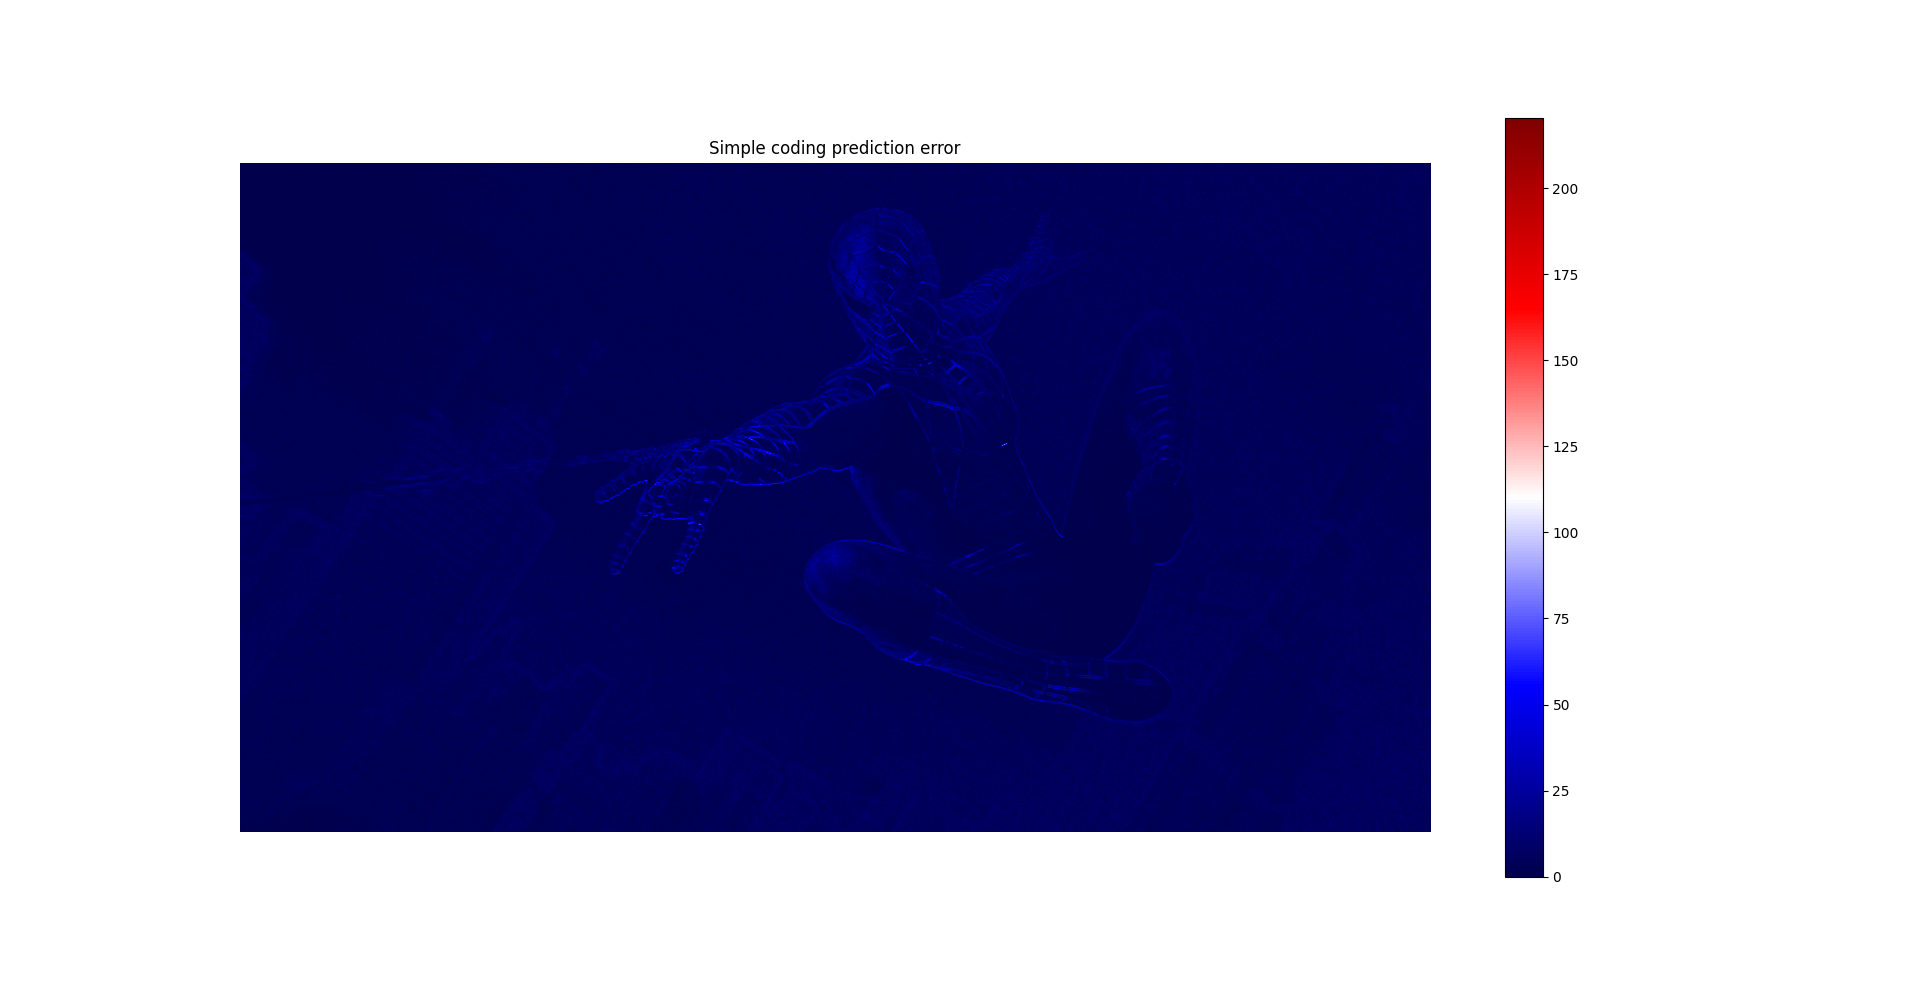
\includegraphics[width = .9\textwidth]{hw-1/report/imgs/simple-coding.png}
    \caption{Rappresentazione del modulo dell'errore di predizione nella codifica semplice.}
    \label{fig:simple-coding}
\end{figure}
Dall'immagine si può notare che le zone più chiare, ovvero le zone in cui il predittore ha fatto più errori, sono le zone dei contorni, in particolare del personaggio raffigurato. Questo perchè la differenza dei colori tra una sezione e l'altra è particolarmente accentuata. D'altro canto, le zone di colore blu scuro sono quelle in cui i colori sono più uniformi: i palazzi e il cielo sono quais dello stesso colore, suggerendo una zona dove la variazione di colore - e quindi di informazione - è molto bassa.



\subsection{Entropia dell'errore di predizione}\label{simple-coding-error-entropy}
La richiesta successiva è quella di calculare il valore dell'entropia dell'errore di predizione $y(n)$. Utilizzando uno script del tutto simile a quello utilizzato nella task \ref{img-entropy} è quindi possibile calcolare l'entropia richiesta.

\begin{lstlisting}
    # count the occurrences of each prediction error value
    occ, _ = np.histogram(simple_coding_error, bins = range(-255, 256))

    # calculate the relative frequencies and remove any probability == 0
    freqRel = occ / np.sum(occ)
    p = freqRel[freqRel > 0]

    # calculate the entropy
    entropy_y = - np.sum(p * np.log2(p))
\end{lstlisting}

\noindent Dopo l'esecuzione dello script si ottiene che l'entropia dell'errore di predizione semplice è \textbf{4.382 bpp}.



\subsection{Codifica esponenziale di Golomb}\label{exp-golomb}
Seguedo le direttive della task numero 7, calcoliamo la codifica esponenziale di Golomb (detta anche \textsl{exp-Golomb}), la quale dato un numero intero ritorna la sua codifica. Quest'ultima è più efficacie riespetto ad una normale codifica binaria in quanto durante la coidifica vengono risparmiati diversi bit, migliorando la compressione. 

Tale codifica può essere esaminata prima affrontando il caso in cui tutti i numeri da codificare siano ineri positivi e poi tale concetto si può generalizzare. La codifica di Golomb per interi positivi, detta anche \textsl{exponential Golomb unsigned}, è deifnita come segue.

\begin{gather*}
    \text{\texttt{eg\_unsigned}}(n) =
    \begin{cases}
        1 \hspace{180px} \text{se } \, n = 0 \\
        \text{zeros}\left( \left\lfloor \log_2(n + 1) \right\rfloor \right) + \text{dec2bin}(n + 1) \hspace{20px} \text{altrimenti}
    \end{cases}
\end{gather*}

\noindent Dove \texttt{zeros(}$k$\texttt{)} indica una funzione che ritorna una stringa di $k$ zeri mentre la funzione \texttt{dec2bin(}$n$\texttt{)} ritorna il valore binario del numero naturale $n$. A questo, dopo aver definito la codifica senza segno, la codifica con segno, detta anche \textsl{exponential Golomb signed}, è immediata:

\begin{gather*}
    \text{\texttt{eg\_signed}}(n) =
    \begin{cases}
        \text{\texttt{eg\_unsigned}}(2n - 1) \hspace{20px} \text{se } \, n > 0 \\
        \text{\texttt{eg\_unsigned}}(-2n) \hspace{28px} \text{altrimenti}
    \end{cases}
\end{gather*}

\noindent Dopo aver definito matematicamente la codifica, è possibile tradurla in due funzioni Python molto seplici, che riassumono esattamente quanto già osservato.

\begin{lstlisting}
    def exp_golomb_signed(n: int) -> str:
        # Computes the Exp-Golomb code for signed integers
        
        if n > 0:
            return exp_golomb_unsigned(2 * n - 1)
            
        return exp_golomb_unsigned(-2 * n)
        

    def exp_golomb_unsigned(n: int) -> str:
        # Computes the Exp-Golomb code for non-negative integers

        # handle the case where N is zero
        if n == 0:
            return '1'
        
        # returns the coded string of bits
        return '0' * int( math.floor( math.log2(n + 1) ) ) + format(n + 1, 'b')
\end{lstlisting}

\noindent Possiamo quindi occuparci di calcolare quanto richiesto dalla consegna. Per calcolare il numero di bit necessari utilizzando la codifica esponenziale di Golomb, è sufficiente calcolare la codifica per ogni errore della predizione semplice. La lunghezza delle codifica di ciascun valore viene sommata ottenendo quindi il numero totale di bit necessari per codificare l'errore. Infine, per ottenere il bitrate di codifica è necessario dividere il numero totali di bit per la grandezza dell'immagine. Il seguente script ricopre esattamente queste direttive.

\begin{lstlisting}
    def exp_golomb_count(vector: list) -> int:
        # Calculate the bitrate based on the exponential Golomb code for a given vector.

        bit_count = 0
        for symbol in vector:
            bit_count += len(exp_golomb_signed(int(symbol)))

        return bit_count

    exp_golomb_bit = exp_golomb_count(simple_coding_error) 

    exp_golomb_bpp = exp_golomb_bit / img_size
\end{lstlisting}

\noindent Dopo l'esecuzione dello script, il numero di bit necessari per la codifica è $41\,305\,140$ mentre il bitrate di codifica ha il valore di \textbf{4.980 bpp}.


\subsection{Conclusioni}
Cerchiamo ora di ottenere dei dati statistici che ci permettano di trarre delle informazioni utili. Si sono scelte sei immagini, mostarte nella figura \ref{fig:all-figures}, alcune delle quali volte propri a testare le capacità della codifica semplice (e poi di quella avanzata). In peritcolare le prime tre immagini hanno peculiartà uniche: la prima, completamente nera, rappresenta l'assenza di entropia, la seconda (la scacchiera) è composta da blocchi mentre la terza rappresenta del rumore Gaussiano, con l'intendo di avere un'immagine con alta entropia. Le altre immagini invece sono normali immagini da comparare.

\begin{figure}[h]
    \centering
    
\includegraphics[width = .3\textwidth]{hw-1/report/imgs/black.png}
    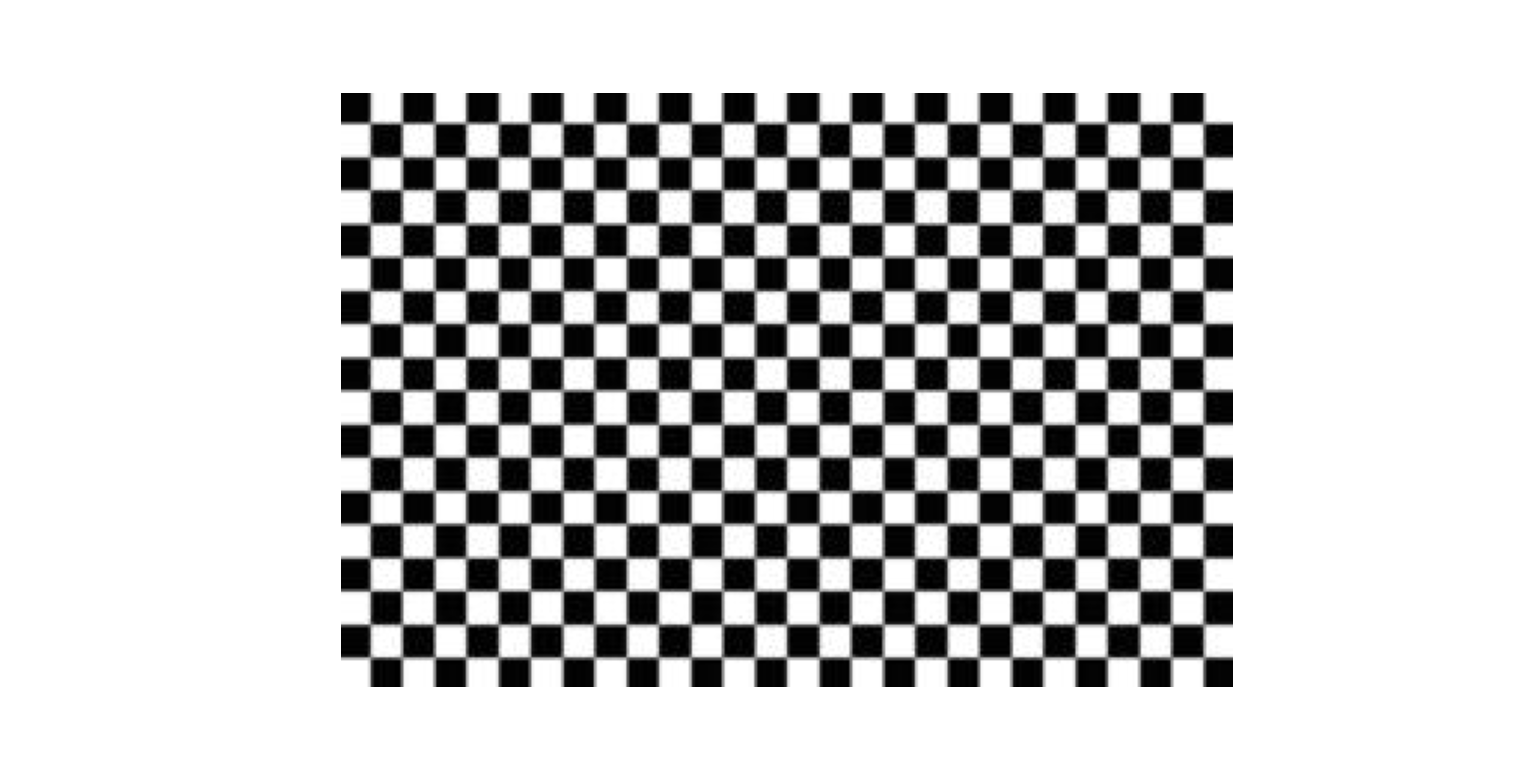
\includegraphics[width = .3\textwidth]{hw-1/report/imgs/chessboard.png}
    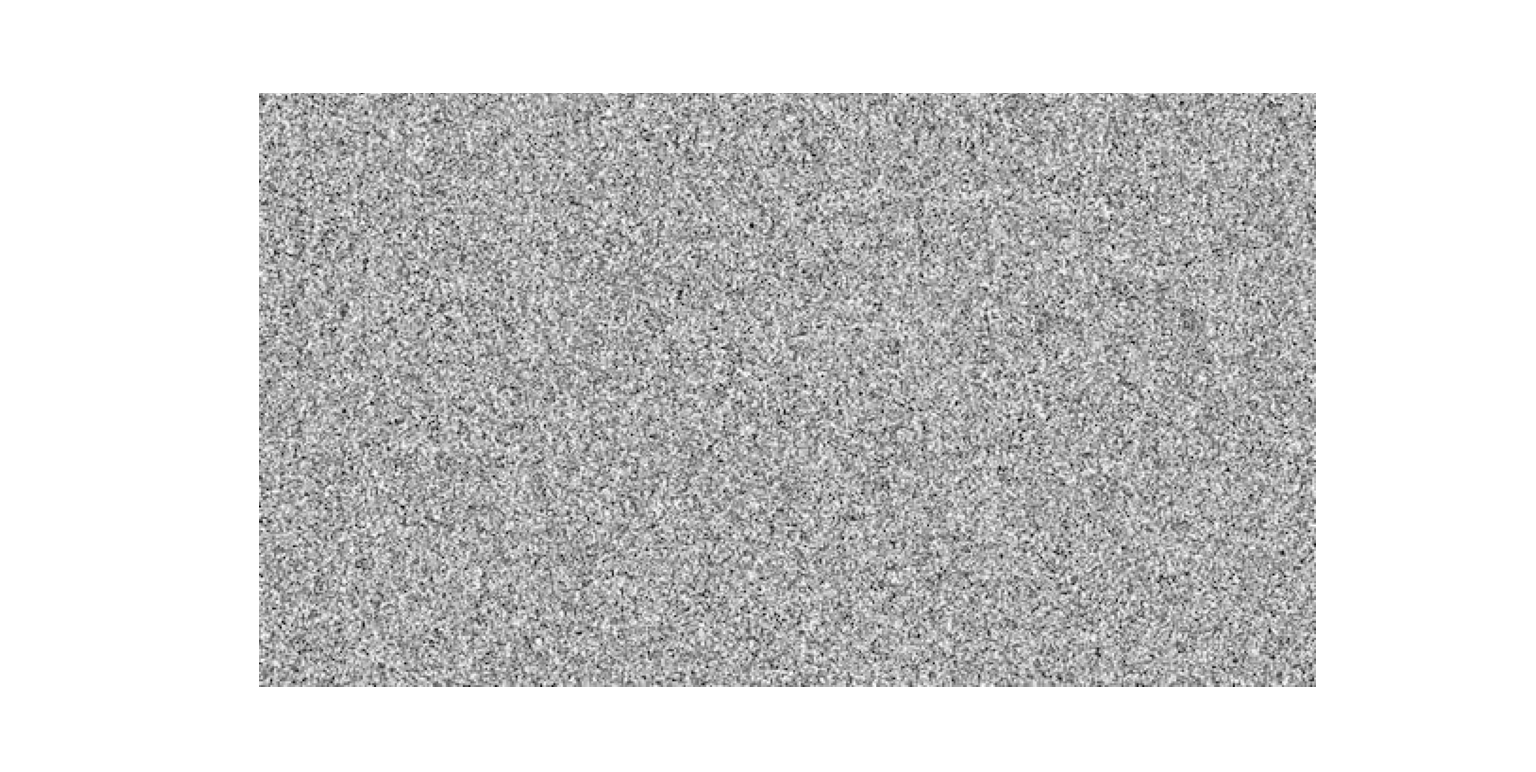
\includegraphics[width = .3\textwidth]{hw-1/report/imgs/gaussian-noise.png}
    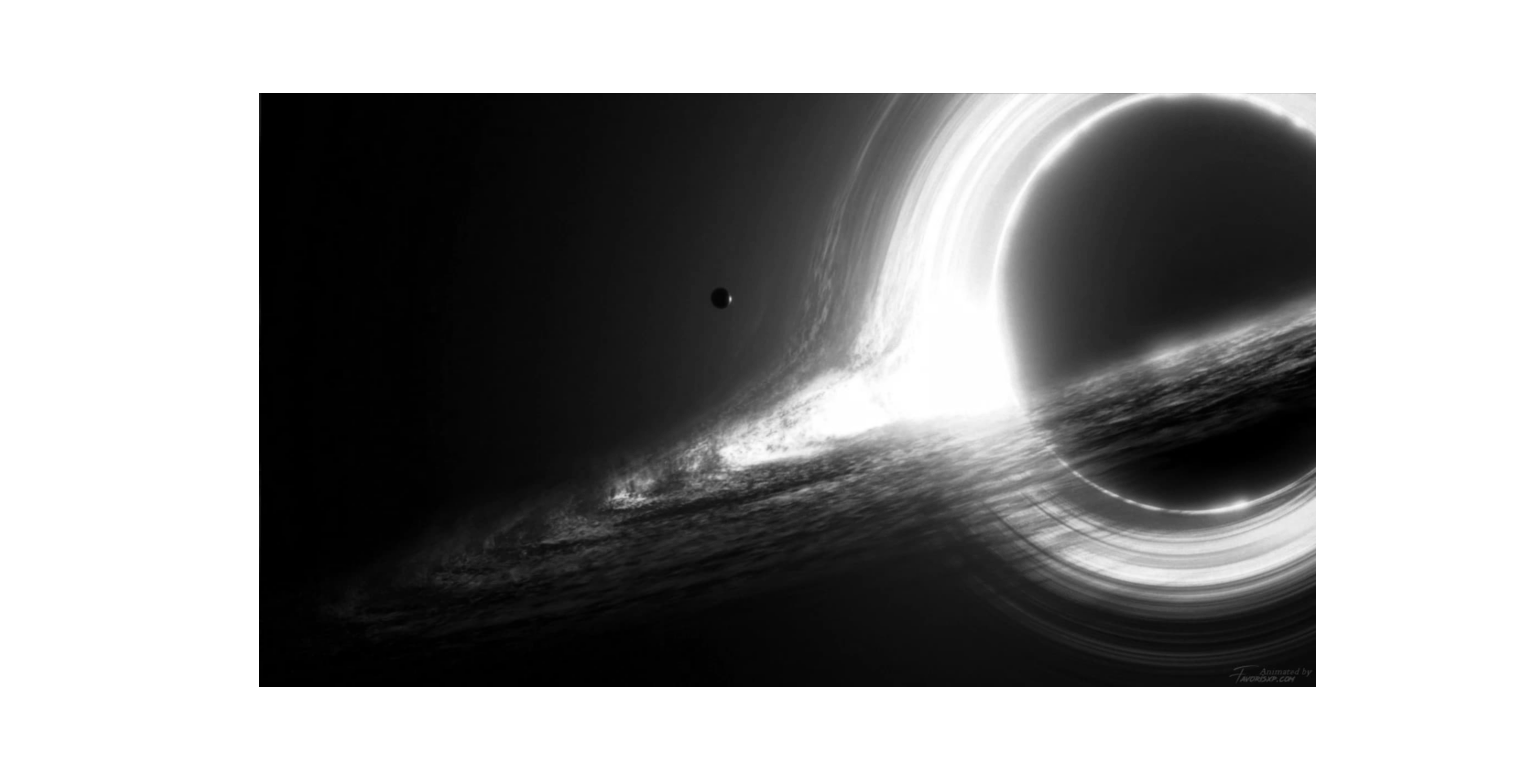
\includegraphics[width = .3\textwidth]{hw-1/report/imgs/interstellar.png}
    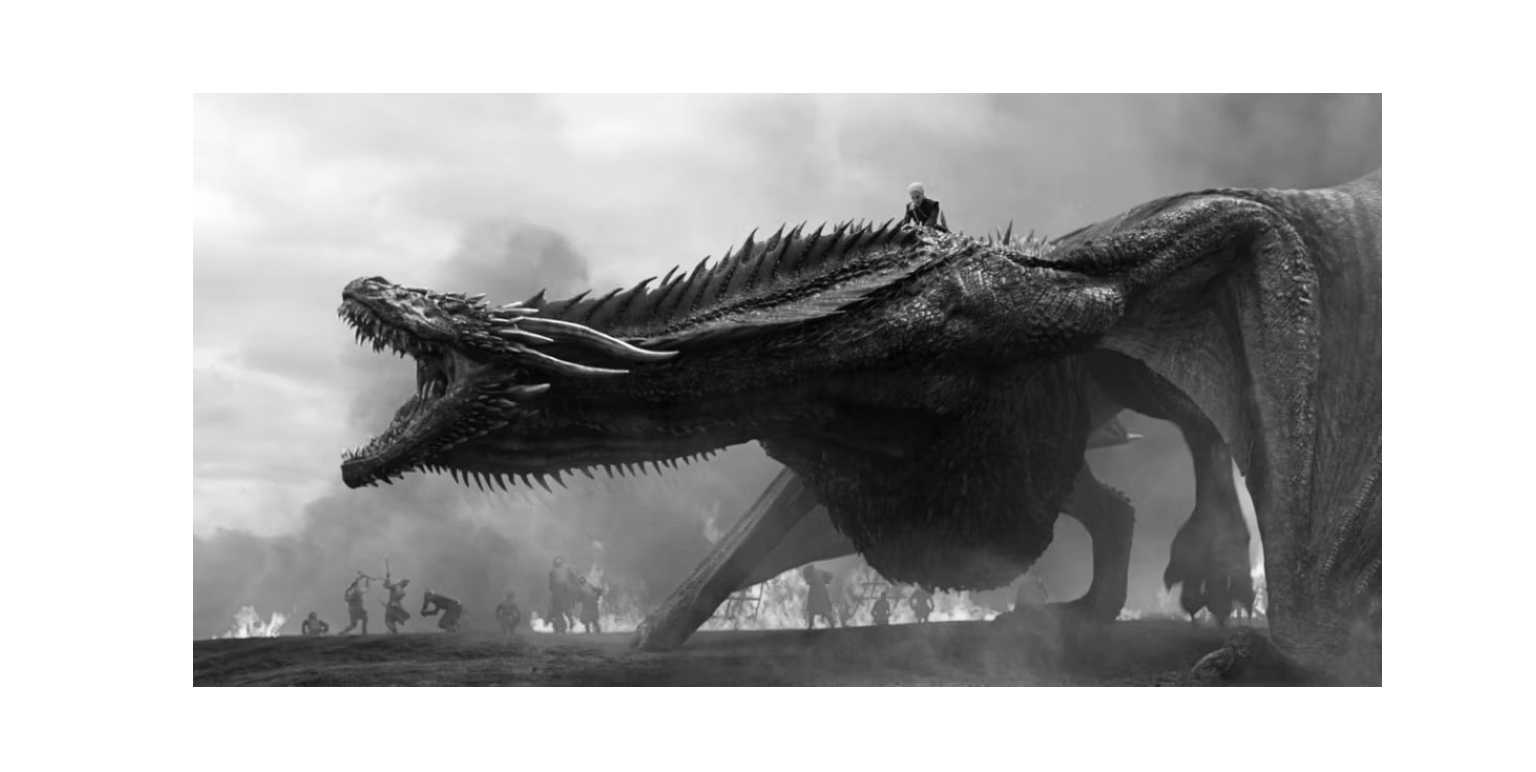
\includegraphics[width = .3\textwidth]{hw-1/report/imgs/dragon.png}
    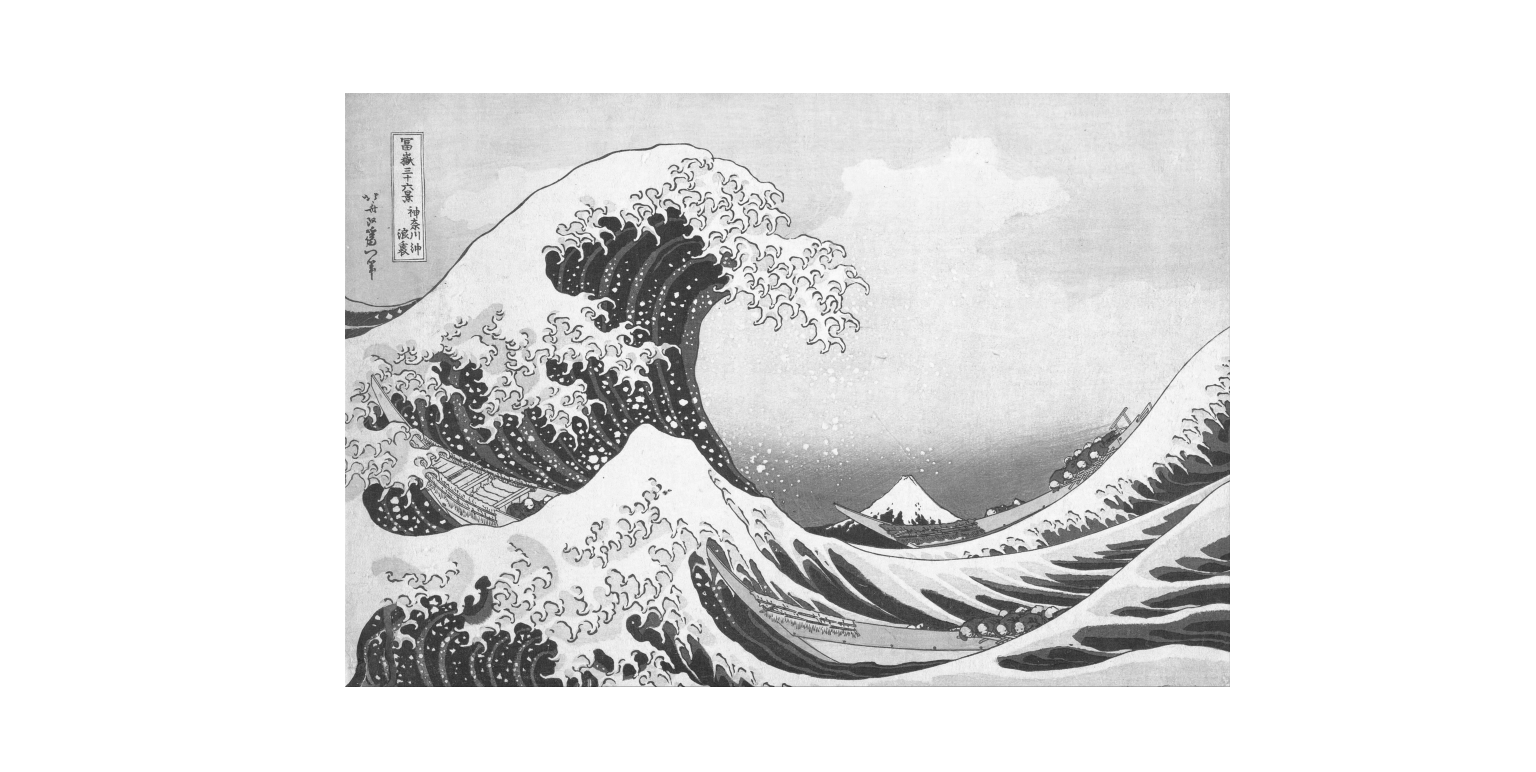
\includegraphics[width = .3\textwidth]{hw-1/report/imgs/great-wave.png}
    \caption{Immagini scelte per effettuare le analisi. }
    \label{fig:all-figures}
\end{figure}


\noindent Per ciascuna delle immagini si è eseguito il codice e i risultati trovati sono stati riassunti nella seguente tabella (\ref{tab:simple-conclusions}).


\begin{table}[h]
    \centering
    \renewcommand{\arraystretch}{1.5}
    \begin{tabular}{| c | c c c c |}
        \hline
        \textbf{img} & \texttt{.pgm} & \texttt{.zip} & \texttt{error} & \texttt{EG-coding} \\ \hline \hline

        black & 0.000 & 0.001 & 0.000 & 1.000 \\
        
        chessboard & 5.539 & 2.218 & 5.420 & 6.364 \\
        
        gaussian-noise & 7.338 & 3.254 & 7.663 & 11.454 \\
        
        interstellar & 6.816 & 0.274 & 2.300 & 2.332 \\
        
        dragon & 7.659 & 1.255 & 3.599 & 3.567 \\
        
        great-wave & 7.055 & 3.022 & 6.175 & 7.947 \\
        
        spiderman & 7.581 & 1.329 & 4.382 & 4.980 \\
        \hline
    \end{tabular}
    \caption{Dati ottenute dalle varie istanze di esecuzione dello script, con immagini diverse.}
    \label{tab:simple-conclusions}
    \renewcommand{\arraystretch}{1}
\end{table}

\noindent Osservando la tebella riassuntiva si possono notare valori particolarmente diversi per ciascuna immagine. Chiaramente l'immagine completamente nera ha entropia nulla e di conseguenza lo è anche l'errore di predizione; anche il tasso di codifica esponensiale di Golomb suggerisce che è  necessario solo un bit per rappresentare l'errore. Per quanto riguarda la seconda immagine, quella della scacchiera, si ha un'entropia più alta ma comunque ridotta rispetto alle altre immagini. Questo perché i due colori dominanti sono il bianco e il nero, senza altre variazioni di conseguenza il segnale non è sparsioficato come negli altri casi. Ciò nonostante il tasso di codifica è comunque abbastanza elevato. Nella terza immagine, raffigurante il rumore Gaussiano, possiamo notare che sia l'entropia, ma ancora di più l'errore di predizione sono molto elevati. Questo perchè i pixel dell'immagine sono casuali rendendolo un segnale difficile da predire. Proprio per questo motivo il suo tasso di codific è così elevato.

Nel caso delle altre immagini, i risultati non sono così inaspettati, a perte nel caso della \textsl{Great wave} dove l'entropia dell'errore di predizione e il tasso di codifica sono comunque particolarmente elevati rispetto alle altre immagini.





\newpage\section{Codifica avanzata}
La seconda parte dell'homewrok richiede di effettuare la modifica avanzata sull'immagine ed analizzarne i risultati. Infine viene richiesto di comprarli con quelli ottenuti nella codifica semplice.


\vspace{15px}\subsection{Codifica avanzata}

La penultima richiesta, esige di creare un nuovo tipo di codifica, detta \textsl{avanzata} definita come segue:

\begin{gather*}
    y(n, m) = 
    \begin{cases}
        x(n, m) - 128 \hspace{161px} \text{se } \, n = m = 0 \\
        x(n, m - 1) \hspace{171px} \text{se } \, n = 0\\
        x(n - 1, m) \hspace{171px} \text{se } \, m = 0\\
        \text{med}\left[ x(n, m - 1),\, x(n - 1, m),\, x(n - 1, m - 1) \right] \hspace{15px} \text{se } \, m = \text{MAX}\\
        \text{med}\left[ x(n, m - 1),\, x(n - 1, m),\, x(n - 1, m + 1) \right] \hspace{15px} \text{altrimenti}
    \end{cases}
\end{gather*} 

\noindent Dove in questo caso l'immagine anzichè essere vista come un vettore $x$ è vista come una matrice di dimensione $n \times m$. Le richieste della codifica sono tradotte in uno script contenente due cicli annidati - il primo che itera lungo le righe della matrice e il secondo che itera lungo le colonne - dove all'intero sono presenti una serie di \texttt{if} statement che soddisfano la definizione di codifica avanzata precedentemente citata. Inoltre si osserva la mediana dei tre valori è calcolata tramite una funzione definita dall'utente, descritta anch'essa all'interno dello script. 

\begin{lstlisting}
    # median function for advanced coding
    def median(a, b, c):
        
        v = [a, b, c]
        v.sort()
    
        return v[1]
    
    
    # codes an image based on the guidelines directives
    def advanced_coding(img):
        # blank image 
        predicted_img = np.zeros_like(img)
        
        # extracts the height and the width from the image
        height, width = img.shape[0], img.shape[1]
    
        # iterates through the rows (height)
        for row in range(height):
    
            # iterates through the cols (width)
            for col in range(width):
    
                if row == 0 and col == 0:   # first pixel
                    predicted_img[row][col] = img[row][col] - 128
                
                elif row == 0:              # first row
                    predicted_img[row][col] = img[row][col - 1]
                
                elif col == 0:              # first col
                    predicted_img[row][col] = img[row - 1][col]
                
                elif col == (width - 1):    # last col
                    predicted_img[row][col] = median(img[row - 1][col], img[row][col - 1], img[row - 1][col - 1])
    
                else:                       # other cases
                    predicted_img[row][col] = median(img[row - 1][col], img[row][col - 1], img[row - 1][col + 1])
    
        return predicted_img


    # performs advanced coding
    predicted_img = advanced_coding(gray_img)

    # calculates the prediction error
    adv_coding_error_img = gray_img - predicted_img
\end{lstlisting}

\noindent Dopo aver eseguito lo script è possibile mostrare l'errore di predizione sottraendo l'immagine predetta \texttt{predicted\_img} con l'immagine iniziale \texttt{img} e "plottando" il suo valore assoluto. L'immagine mostrata in figura \ref{fig:advanced-coding} è ciò che risulta degli errori commessi durante la predizione.

\begin{figure}[h]
    \centering
    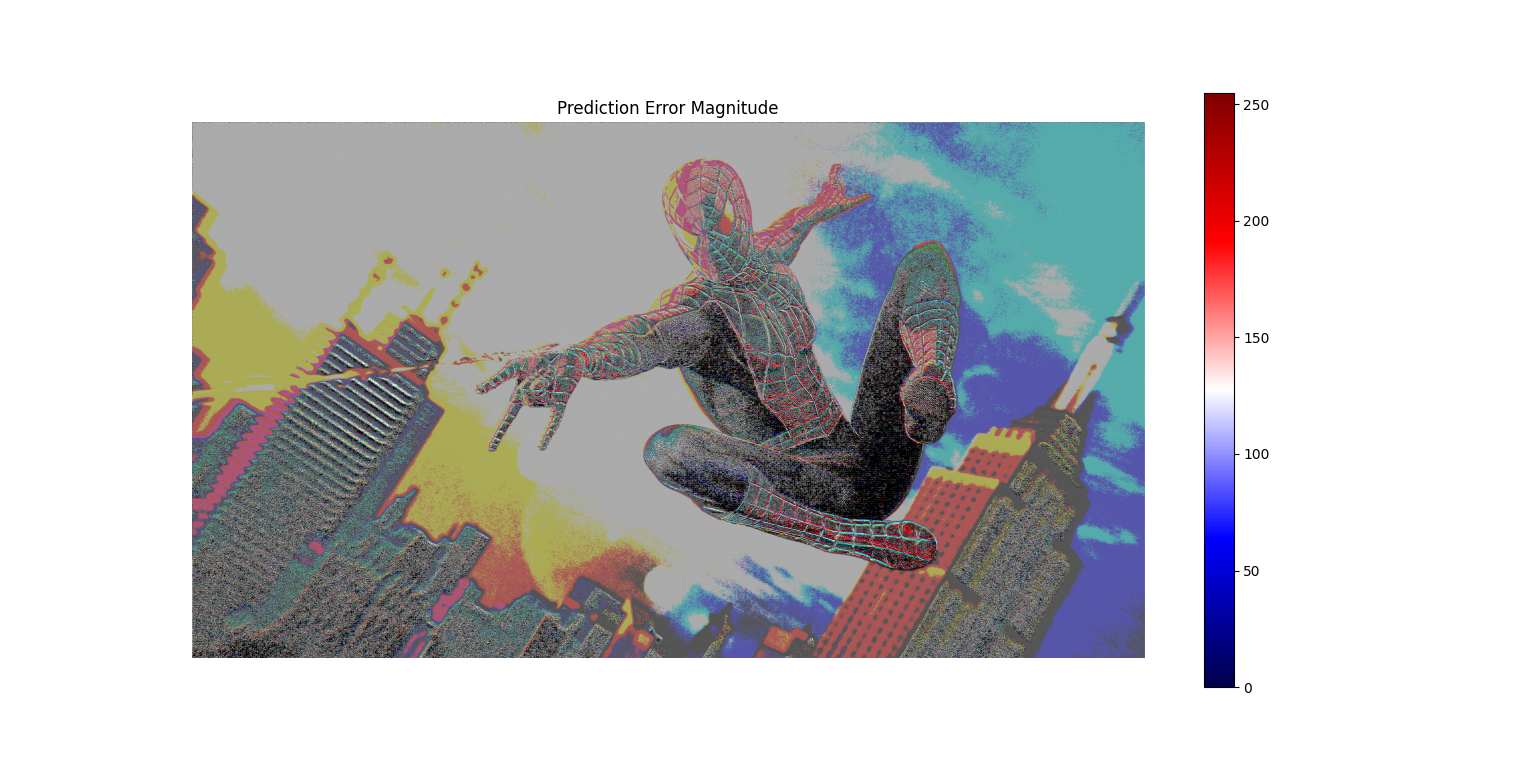
\includegraphics[width = .9\textwidth]{hw-1/report/imgs/advanced-coding.png}
    \caption{Rappresentazione del modulo dell'errore di predizione nella codifica avanzata.}
    \label{fig:advanced-coding}
\end{figure}

\FloatBarrier\noindent Si osserva che per quanto l'immagine \ref{fig:advanced-coding} sia simile alla figura \ref{fig:simple-coding}, è presente una differenza: è sufficente mostrare un'immagine che contenga la differenza in modulo tra le varaibili \texttt{simple\_coding\_error} e \texttt{adv\_coding\_error}. Dal risultato, mostrato nella figura \ref{fig:error-difference}, si può notare che non è di colore uniforme ma presenta diverse sfumature di blu, suggerendo quindi una differenza tra le due immagini di errore.

\begin{figure}[h]
    \centering
    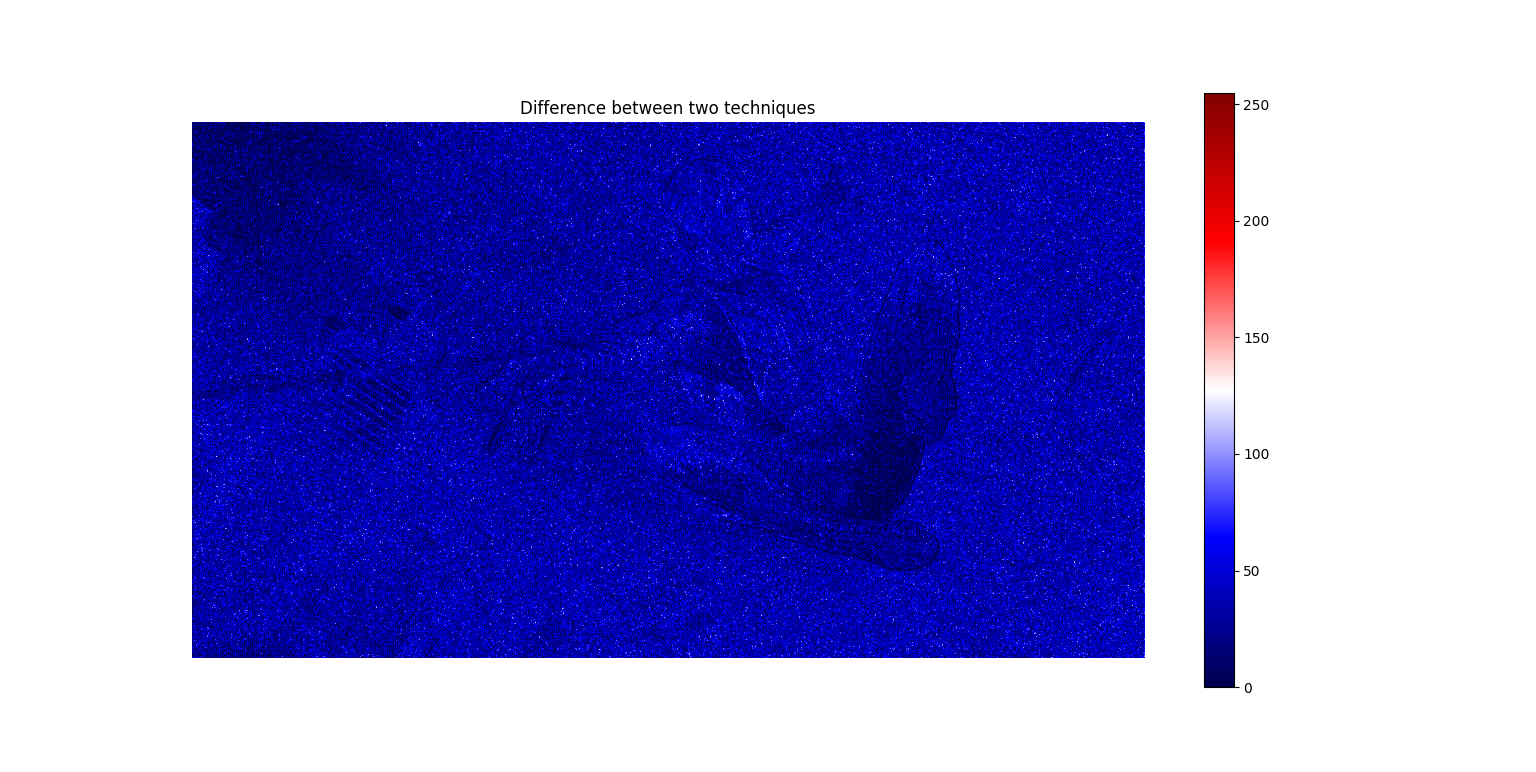
\includegraphics[width = .9\textwidth]{hw-1/report/imgs/error-difference.png}
    \caption{Rappresentazione della differenza tra l'errore della codifica semplice e della codifica avazata.}
    \label{fig:error-difference}
\end{figure}



\vspace{15px}\subsection{Entropia dell'errore di predizione}
Dopo aver calcolato l'errore del predittore avanzato dell'immagine, è necessario calcolarne l'entropia. Le istruzioni necessarie per il calcolo dell'entropia sono le stesse utilizzate per il calcolo dell'entropia del predittore semplice nel pargarfo \ref{simple-coding-error-entropy}.



\begin{lstlisting}
    occ, _ = np.histogram(adv_coding_error_img, bins = range(-255, 256))

    # calculate the relative frequencies and remove any probability == 0
    freqRel = occ / np.sum(occ)
    p = freqRel[freqRel > 0]

    # calculate the entropy
    entropy_y = - np.sum(p * np.log2(p))
\end{lstlisting}

\noindent Dopo aver eseguito lo script, si ottene il valore dell'entropia del valore di predizione avcanzata il quale corrisponde a \textbf{4.195 bpp}, che è minore rispetto a quello ottenuto nell'errore di codifica semplice, suggerendo che la codifica avanzata è stata più efficacie.



\vspace{15px}\subsection{Codifica esponenziale di Golomb}
Come per la codifica semplice, anche in questo caso è necessario calcaolare la codifica esponenziale di Golomb sull'errore di predizione. Il codice utilizzato è esattamente lo stesso indicato sul paragrafo \ref{exp-golomb} con l'unica differenza che la funzione viene invocata sull'errore di predizione avanzata anzichè su quella semplice.

\begin{lstlisting}
    # calculates EG bits
    exp_golomb_bit = exp_golomb_count(adv_coding_error_img.flatten())
    
    # camputes the bitrate
    exp_golomb_bpp = exp_golomb_bit / img_size
\end{lstlisting}

\noindent In questo caso, per l'errore di predizione avanzata sull'immagine \ref{fig:colored-grayscale}, il numero di bit di necessari è di $38\,854\,794$ mentre il bitrate è \textbf{4.6845 bpp}, il quale, anche in questo caso, è minore rispetto a quello della codifica semplice. 



\vspace{15px}\subsection{Confronto con codifica semplice}
% Confrontare l’entropia e il tasso di codifica ottenuti con l’entropia dell’immagine e con il tasso di codifica dell’applicazione zip

Confrontando i valori ottenuti con la codifica avanzata con i valori della codifica semplice, si desume che le prestazioni della codifica avanzata sono migliori. In particolare, per quanto riguarda l'entropia dell'errore, si ha che nella codifica semplice l'entropia è di 4.382 bpp mentre nella codifica avanzata l'entropia corrisponde a 4.195 bpp. Questa differenza indica che la codifica avanzata ha una maggiore efficienza nella riduzione dell'errore di predizione che si traduce in una migliore rappresentazione dell'immagine originale.

In secondo luogo, si nota che anche il tasso di codifica si riduce tra la codifica semplice (che è di 4.980 bpp) e la codifca avanzata (4.685) sottolineando l'efficacia di quest'ultima. La differenza dei due valori indica che con la codifica avanzata si è in grado di rappresentare lo stesso numero di informazioni attraverso un numero minore di bit (infatti $38\,854\,794 < 41\,305\,140$).

Per quanto il tasso di codifica sia largamente minore rispetto all'entropia dell'immagine originale (7.581 bpp), rimane comunque molto più elevato rispetto al \textsl{bitrate} ottenuto zippando l'immagine (che corrispnde a 1.329 bpp). Questo è dovuto al fatto che la codifica avanzata implementata rimane comunque molto meno inefficiente rispetto alle tecniche ottimizzate della codifica con dizionario offerta dai sistemi operativi.






\vspace{15px}\section{Conclusioni}

\todo{inserisci discussione finale sulla differenza dei valori trovati}



\begin{figure}[h]
    \centering
    
\includegraphics[width = .3\textwidth]{hw-1/report/imgs/black.png}
    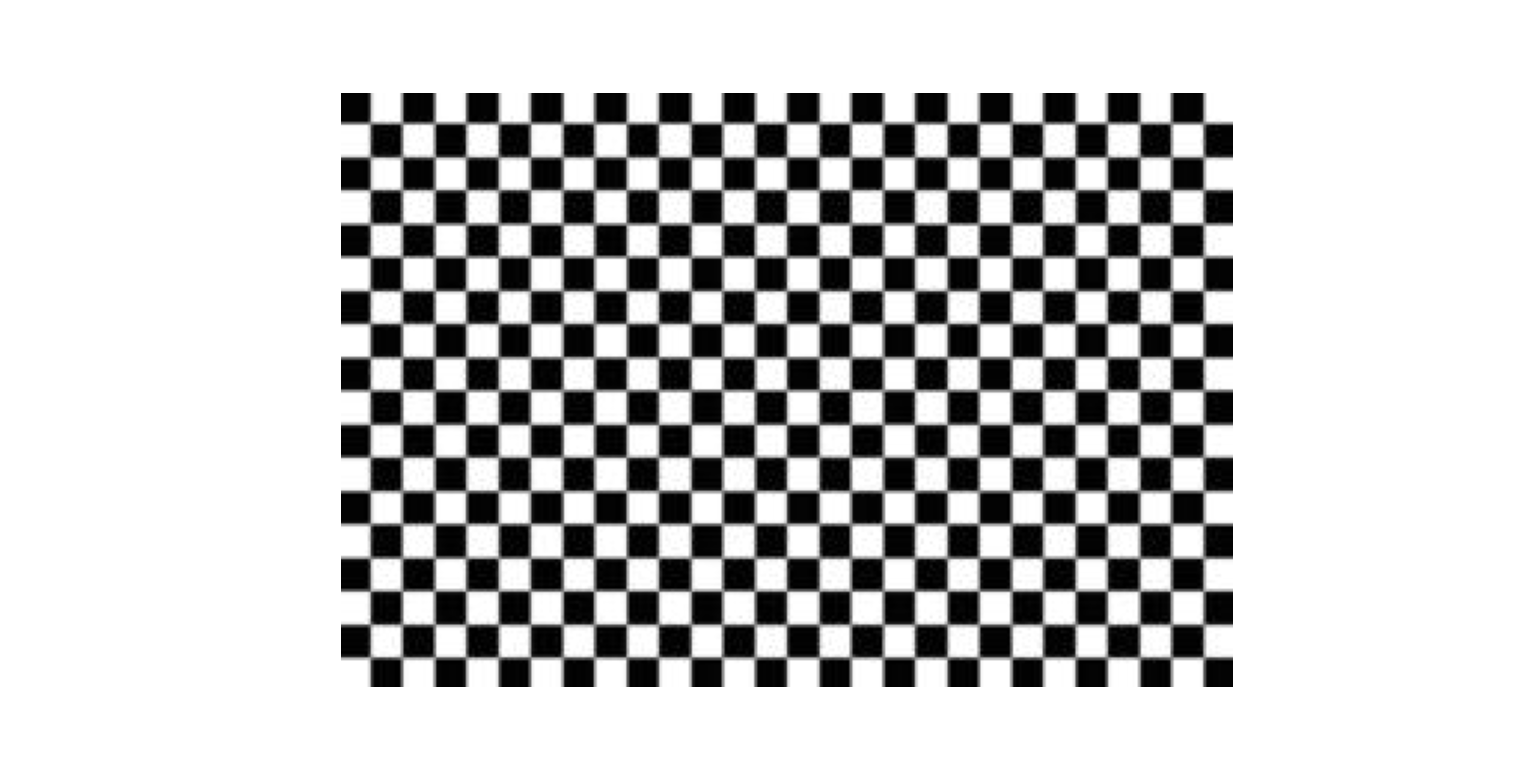
\includegraphics[width = .3\textwidth]{hw-1/report/imgs/chessboard.png}
    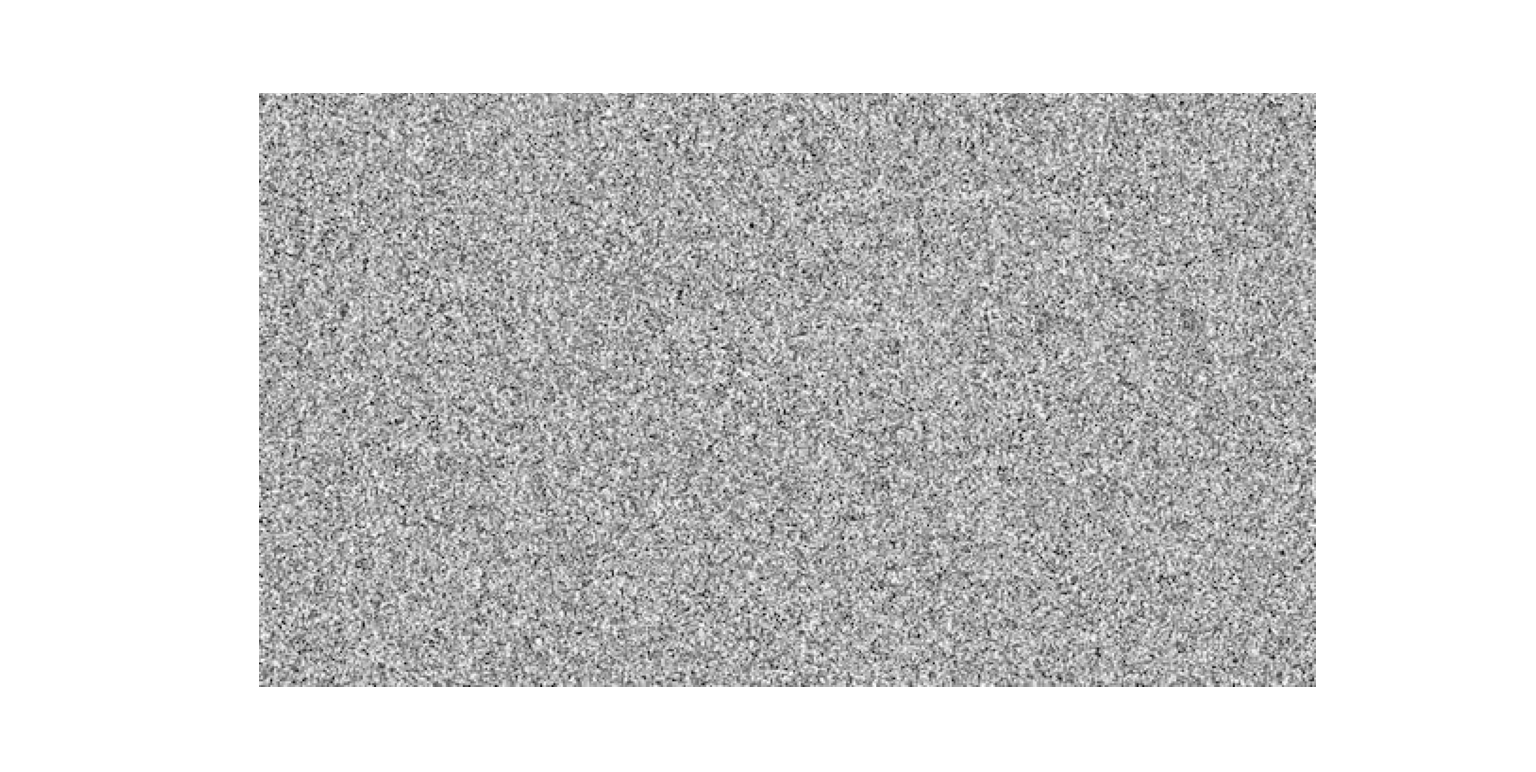
\includegraphics[width = .3\textwidth]{hw-1/report/imgs/gaussian-noise.png}
    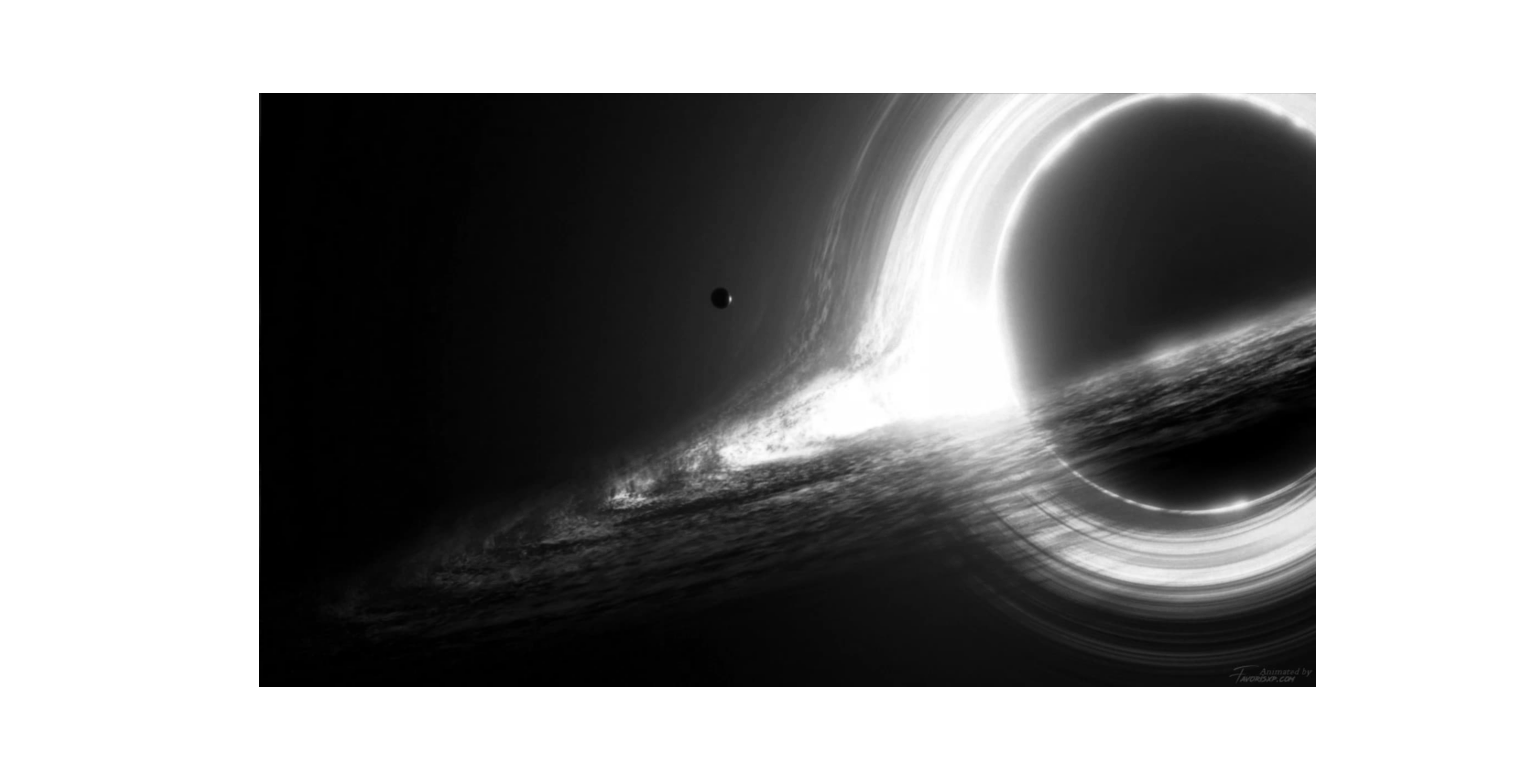
\includegraphics[width = .3\textwidth]{hw-1/report/imgs/interstellar.png}
    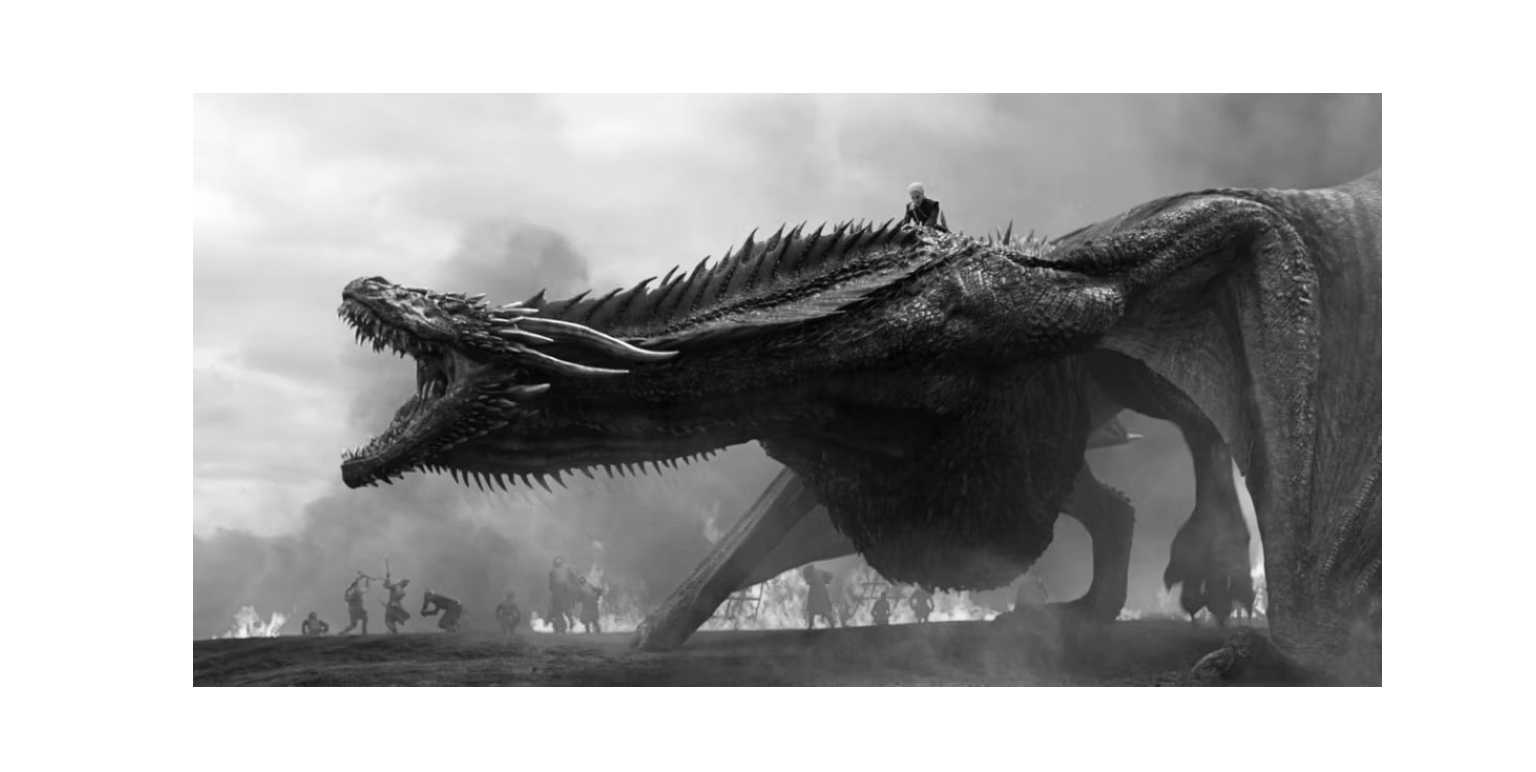
\includegraphics[width = .3\textwidth]{hw-1/report/imgs/dragon.png}
    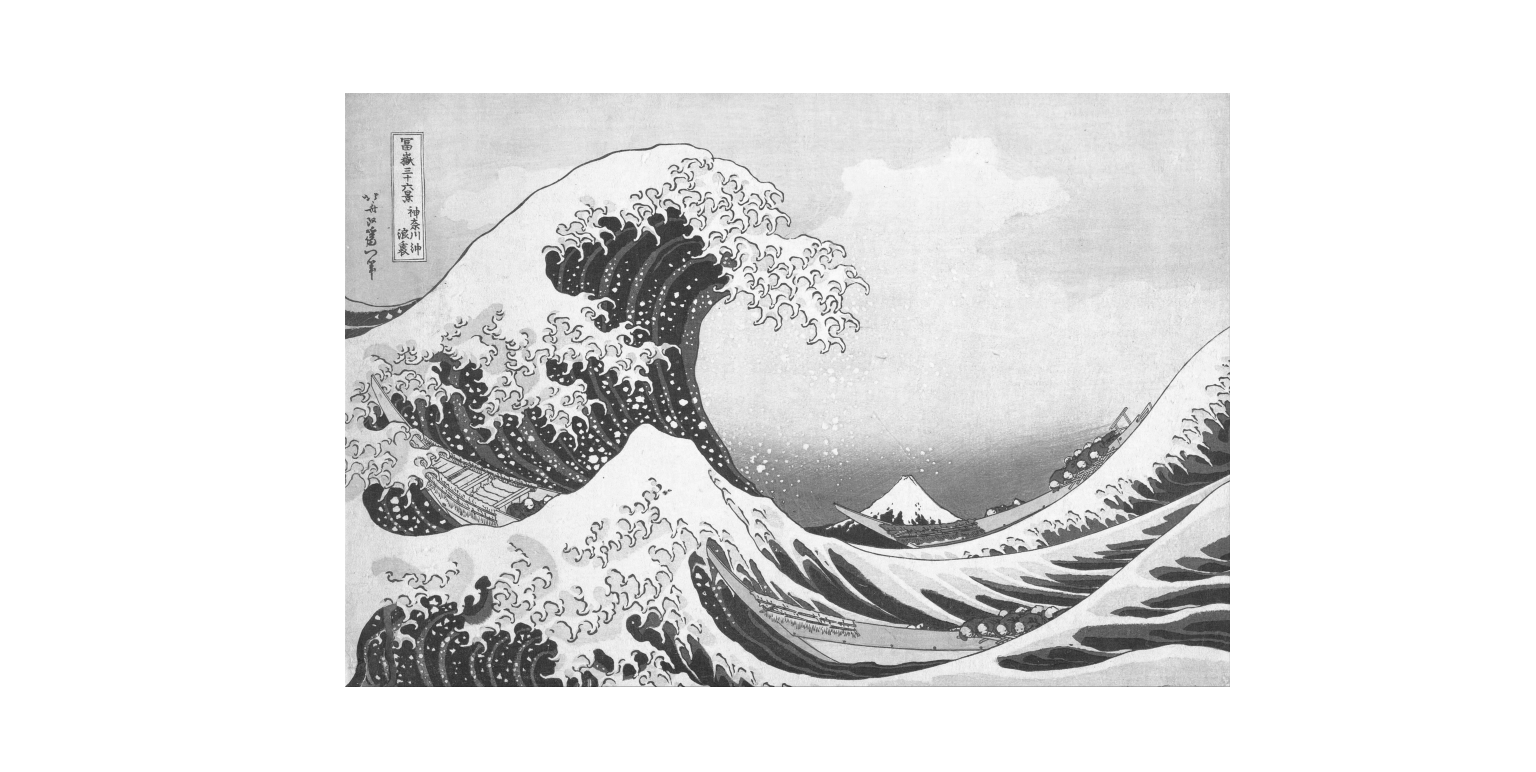
\includegraphics[width = .3\textwidth]{hw-1/report/imgs/great-wave.png}
    \caption{Immagini scelte per effettuare le analisi. }
    \label{fig:all-figures-final}
\end{figure}




\begin{table}[h]
    \centering
    \renewcommand{\arraystretch}{1.5}
    \begin{tabular}{| c | c c | c c |}
        \hline
        \multirow{2}{*}{Immagine} & \multicolumn{2}{c|}{\textbf{Entropia}} & \multicolumn{2}{c|}{\textbf{Tasso di codifica}} \\
        & Semplice & Avanzata & Semplice & Avanzata \\\hline\hline

        black & 0.000 & 0.000 & 1.000 & 1.000 \\
        
        chessboard & 5.420 & 5.529 & 6.364 & 6.457 \\
        
        gaussian-noise & 7.663 & 7.459 & 11.454 & 11.092 \\
        
        interstellar & 2.300 & 2.139 & 2.332 & 2.177 \\
        
        dragon & 3.599 & 3.412 & 3.567 & 3.338 \\
        
        great-wave & 6.175 & 6.056 & 7.947 & 7.801 \\
        
        spiderman & 4.382 & 4.195 & 4.980 & 4.684\\
        \hline
    \end{tabular}
    \caption{Tabella riassuntiva.}
    \label{tab:overall-conclusions}
    \renewcommand{\arraystretch}{1}
\end{table}

\todo{Focalizza l'attenzion su chessboard, dove la differenza del predittore e maggiore perche si basa anmche sulle celle sopra e non solo sdu quelle a destra}

\end{document}
